\documentclass{beamer}

\usepackage[T1]{fontenc}
\usepackage[latin1]{inputenc}
\usepackage{lmodern}
\usepackage{amsmath,amssymb,amsthm}
\usepackage{graphicx}
\usepackage{tcolorbox}
\usepackage{listings}

\usetheme[headline=section, footlineleft=empty, footlinecenter=empty, footlineright=frames]{TUMCD}
\usefonttheme{professionalfonts}

\lstset{frame=tb, language=Java, aboveskip=3mm, belowskip=3mm, showstringspaces=false, columns=flexible, basicstyle={\small\ttfamily}, numbers=none, numberstyle=\tiny\color{gray}, keywordstyle=\color{blue}, commentstyle=\color{dkgreen}, stringstyle=\color{mauve}, breaklines=true, breakatwhitespace=true, tabsize=3}

\begin{document}

\section{Developed Model}

\begin{frame}
    \frametitle{Discretization of the ODE}

    Discretize time interval:
    \begin{align*}
        &[0,T] \rightarrow \left\{ 0=t_0, t_1, \dots, t_{m-1}, t_{m}=T 
        \right\} \\
    \end{align*}

    Discretize state and control:
    \begin{align*}
        &x_n = x(t_n) \\
        &u_n = u(t_n) \\
    \end{align*}
\end{frame}

\begin{frame}
    \frametitle{Discretization of the ODE}

    Explicit Euler for every time step $h_n=t_{n+1}-t_n$:
    \begin{align*}
        &x_{n+1} \approx \tilde{x}_{n+1} = x_n + h_n f(x_n,u_n,p) =: \Psi(x_n,u_n,p) \\
    \end{align*}

    Discrete constraint:
    \begin{align*}
        &0 = x_{n+1} - \Psi(x_n,u_n,p) =: \Phi_n(x,u,p) \quad \forall n = 0,\ldots,m-1
    \end{align*}
\end{frame}



\begin{frame}
    \frametitle{Problem Formulation}
    Natural approach: Optimal Control Problem
    \begin{align*}
        \min_{x,p} & & \frac{1}{2} \| \bar{x} - x \|^2 & & \\
        \operatorname{s.t.} & & \Phi(x,u,p) & = 0 & & \\
                            & & p & \geq 0 & & \\
    \end{align*}

    \begin{tabular}{ll}
        state & $ x = (s,\theta,\dot{s},\dot{\theta})^T $ \\
        control & $ u = (\tau_1,\tau_2)^T $ \\
        parameters & $ p = (p_1,...,p_k)^T $ \\
        desired motion & $\bar{x}$ \\
    \end{tabular}
\end{frame}

\begin{frame}
    \frametitle{Problem Formulation}
    Input:
    \begin{itemize}
        \item{control $u$}
        \item{desired motion $\bar{x}$ related to $u$}
    \end{itemize}

    Output:
    \begin{itemize}
        \item{parameters $p$ of the excavator}
        \item{x, but not of interest}
    \end{itemize}

    Idea:
    \begin{itemize}
        \item{get rid of variable $x$}
        \item{set $x := \bar{x}$}
        \item{solve a relaxed problem}
    \end{itemize}
\end{frame}

\begin{frame}
    \frametitle{Problem Formulation}

    Original Problem
    \begin{align*}
        \min_{x,p} & & \frac{1}{2} \| \bar{x} - x \|^2 & & \\
        \operatorname{s.t.} & & \Phi(x,u,p) & = 0 & & \\
                            & & p & \geq 0 & & \\
    \end{align*}

    Reinterpreted Problem
    \begin{align*}
        \min_{p}  & & \frac{1}{2} \| \Phi(\bar{x},u,p) \|^2 & & \\
        \operatorname{s.t.} & & p & \geq 0 & & \\
    \end{align*}
\end{frame}

\begin{frame}
    \frametitle{Results}
        Without approximation error

        x(p) solution of ODE using parameters p

        Explicit Euler

    \begin{columns}[t]
        \column{.5\linewidth}
            \begin{figure}
                \centering
                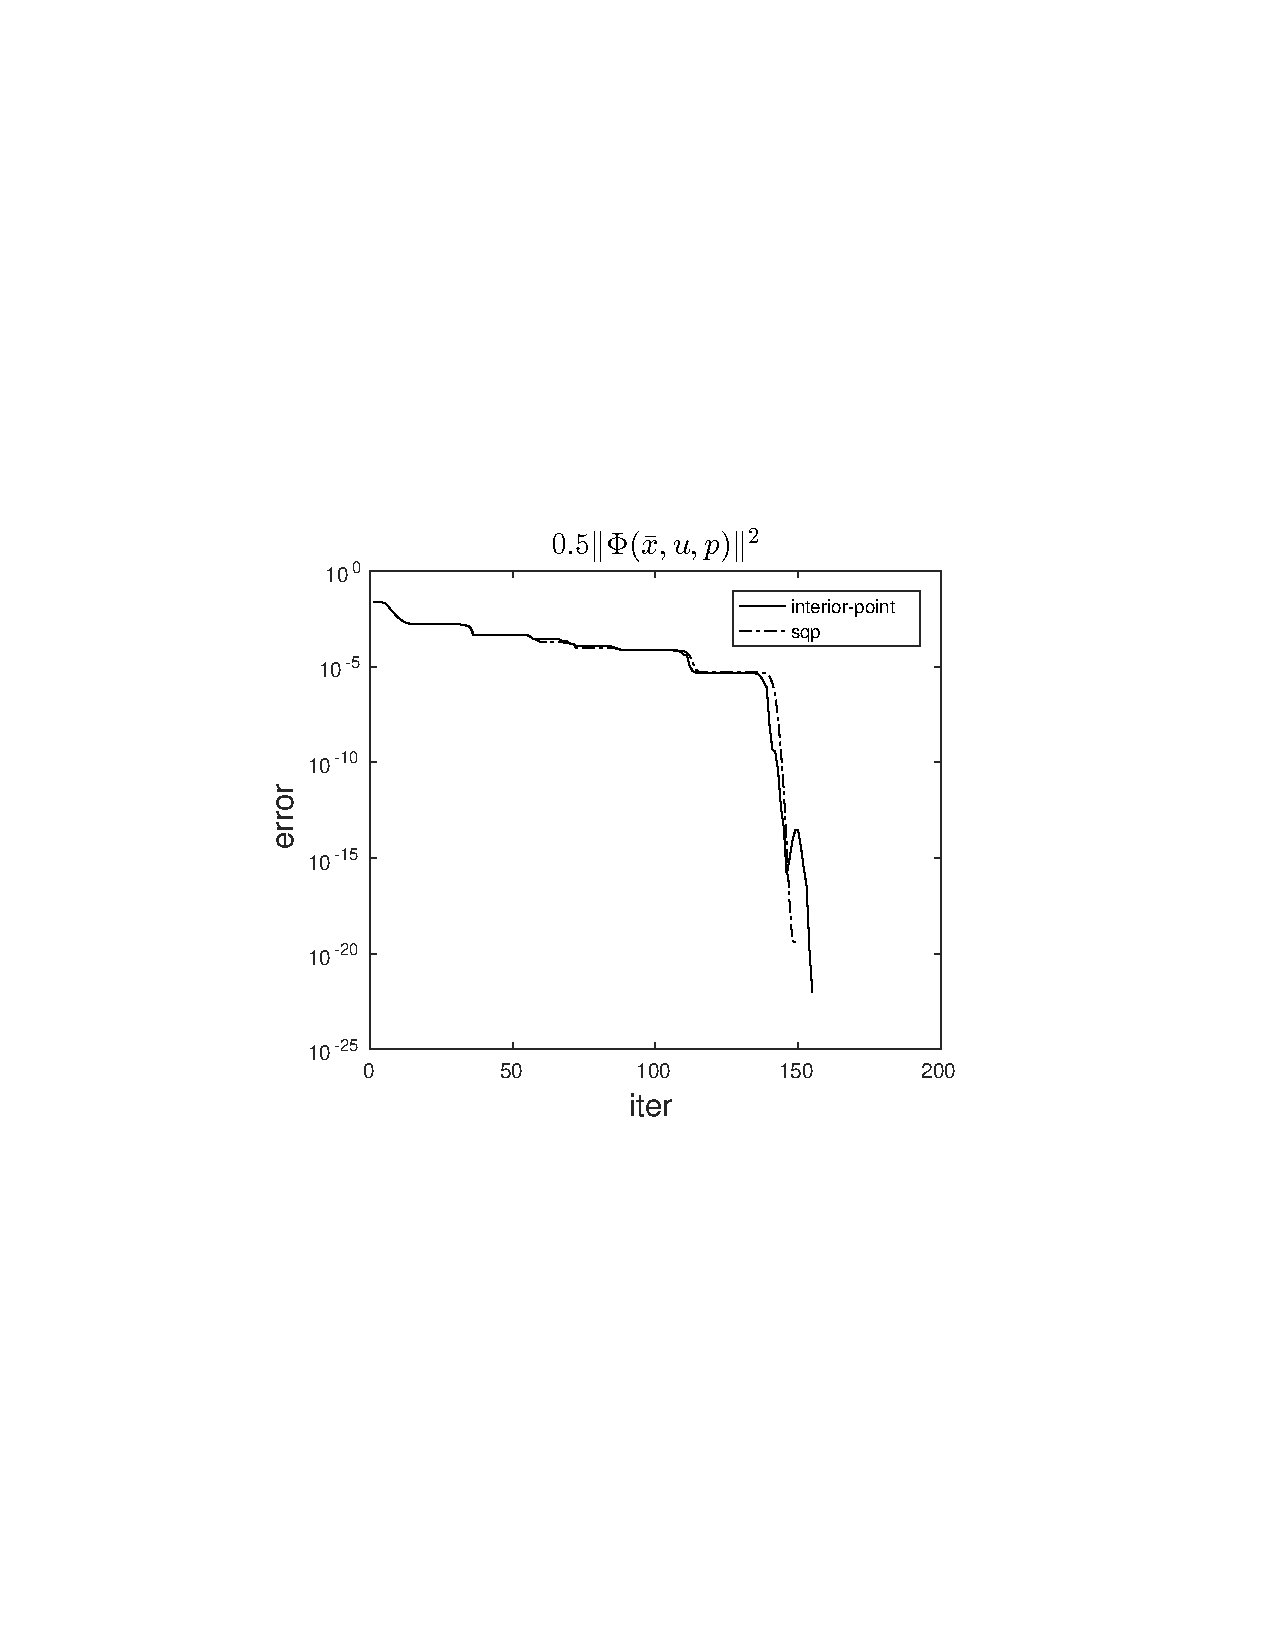
\includegraphics[trim=4cm 9cm 4cm 8.5cm, clip=true, width=\linewidth]{img/convPlotPhi_ref2}
            \end{figure}
        \column{.5\linewidth}
            \begin{figure}
                \centering
                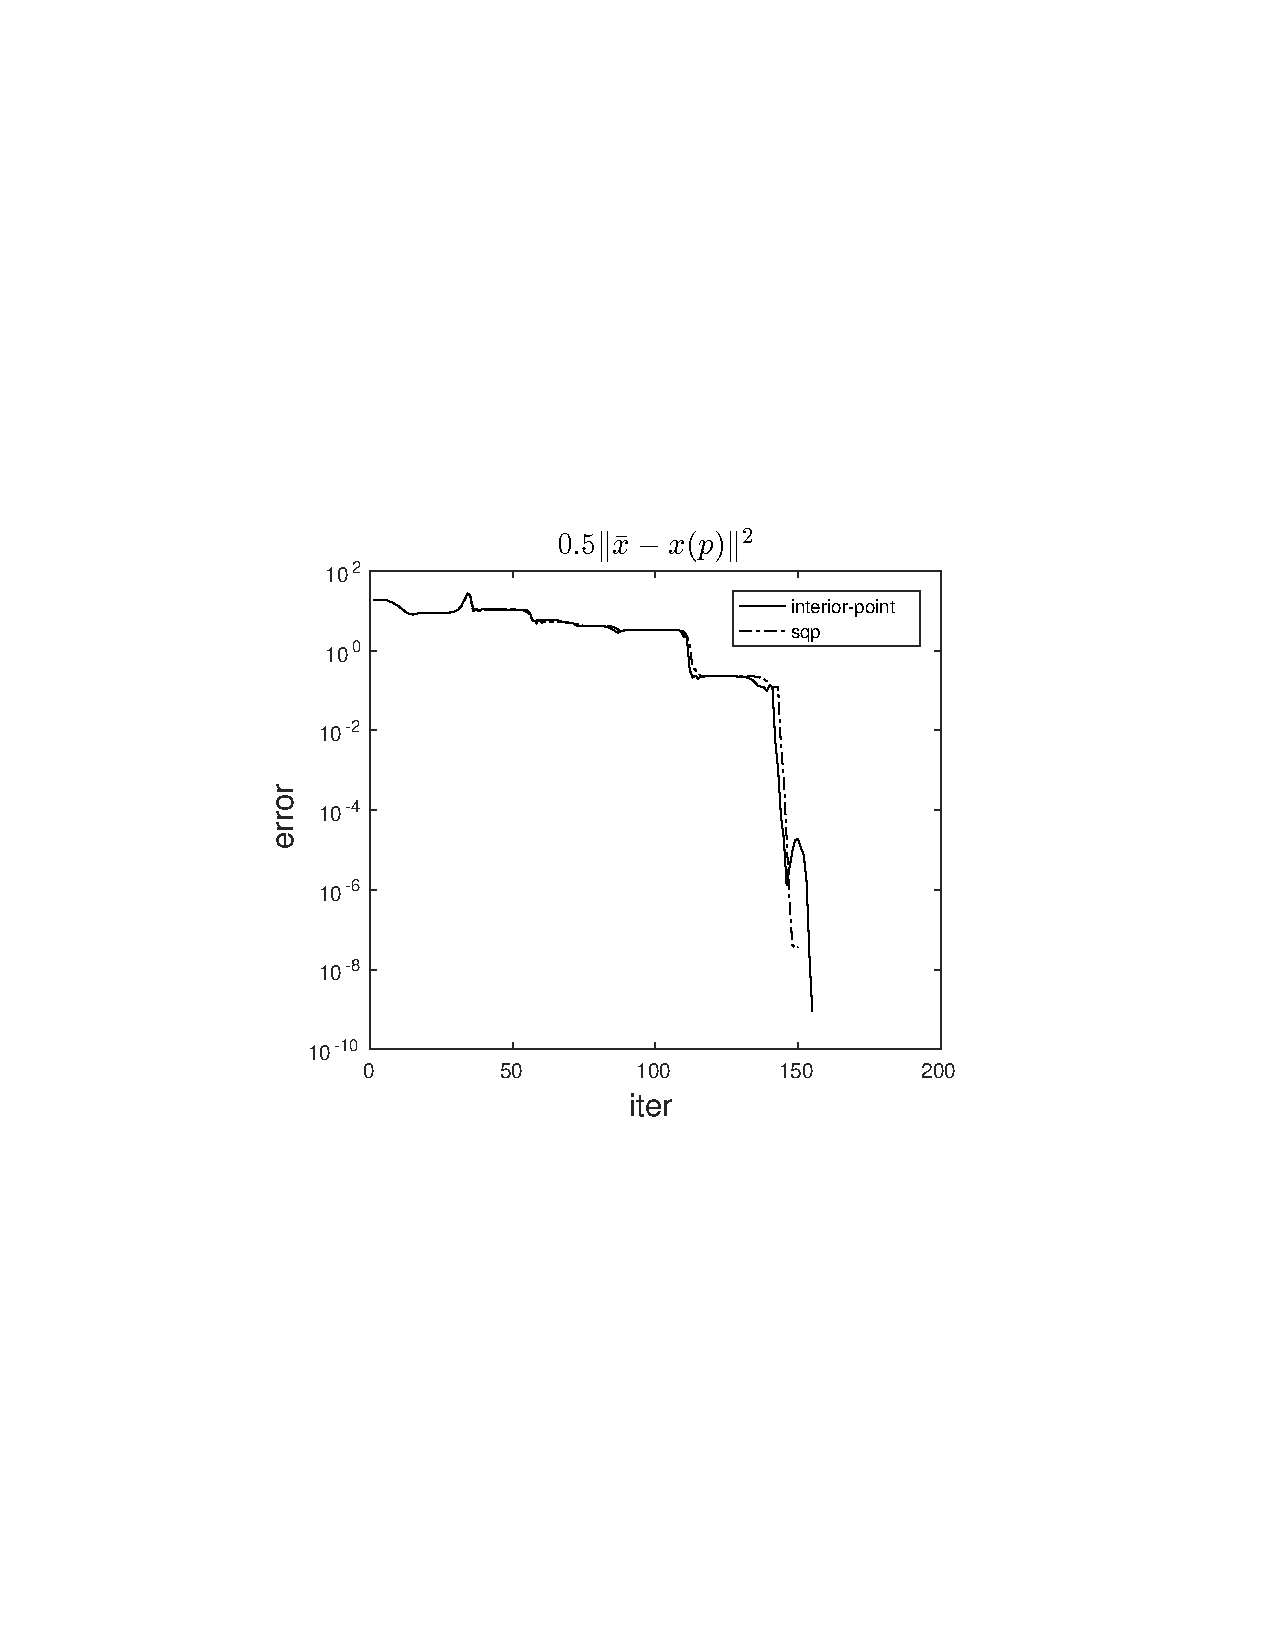
\includegraphics[trim=4cm 9cm 4cm 8.5cm, clip=true, width=\linewidth]{img/convPlotX_ref2}
            \end{figure}
    \end{columns}
\end{frame}

\begin{frame}
    \frametitle{Results}

    \begin{columns}[t]
        \column{.5\linewidth}
            \begin{figure}
                \centering
                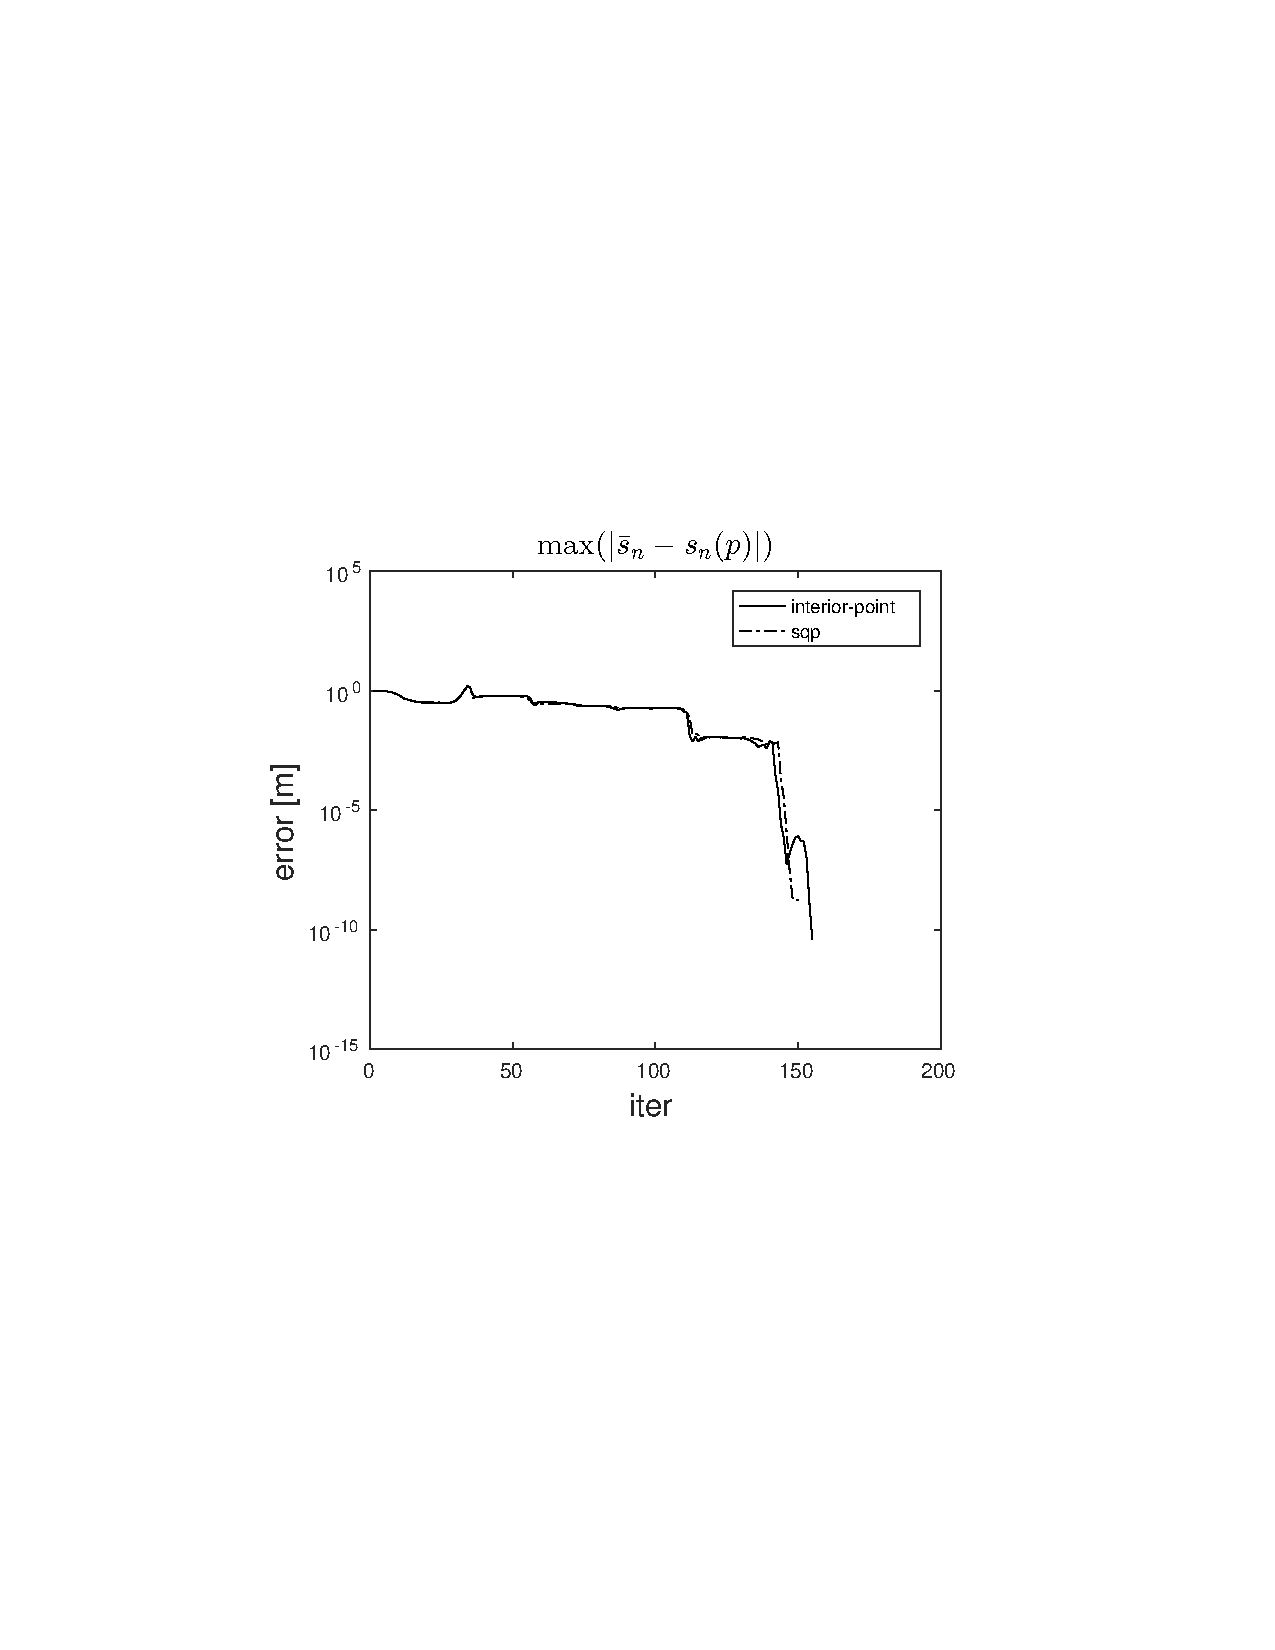
\includegraphics[trim=4cm 9cm 4cm 8.5cm, clip=true, width=\linewidth]{img/convPlotS_ref2}
            \end{figure}
        \column{.5\linewidth}
            \begin{figure}
                \centering
                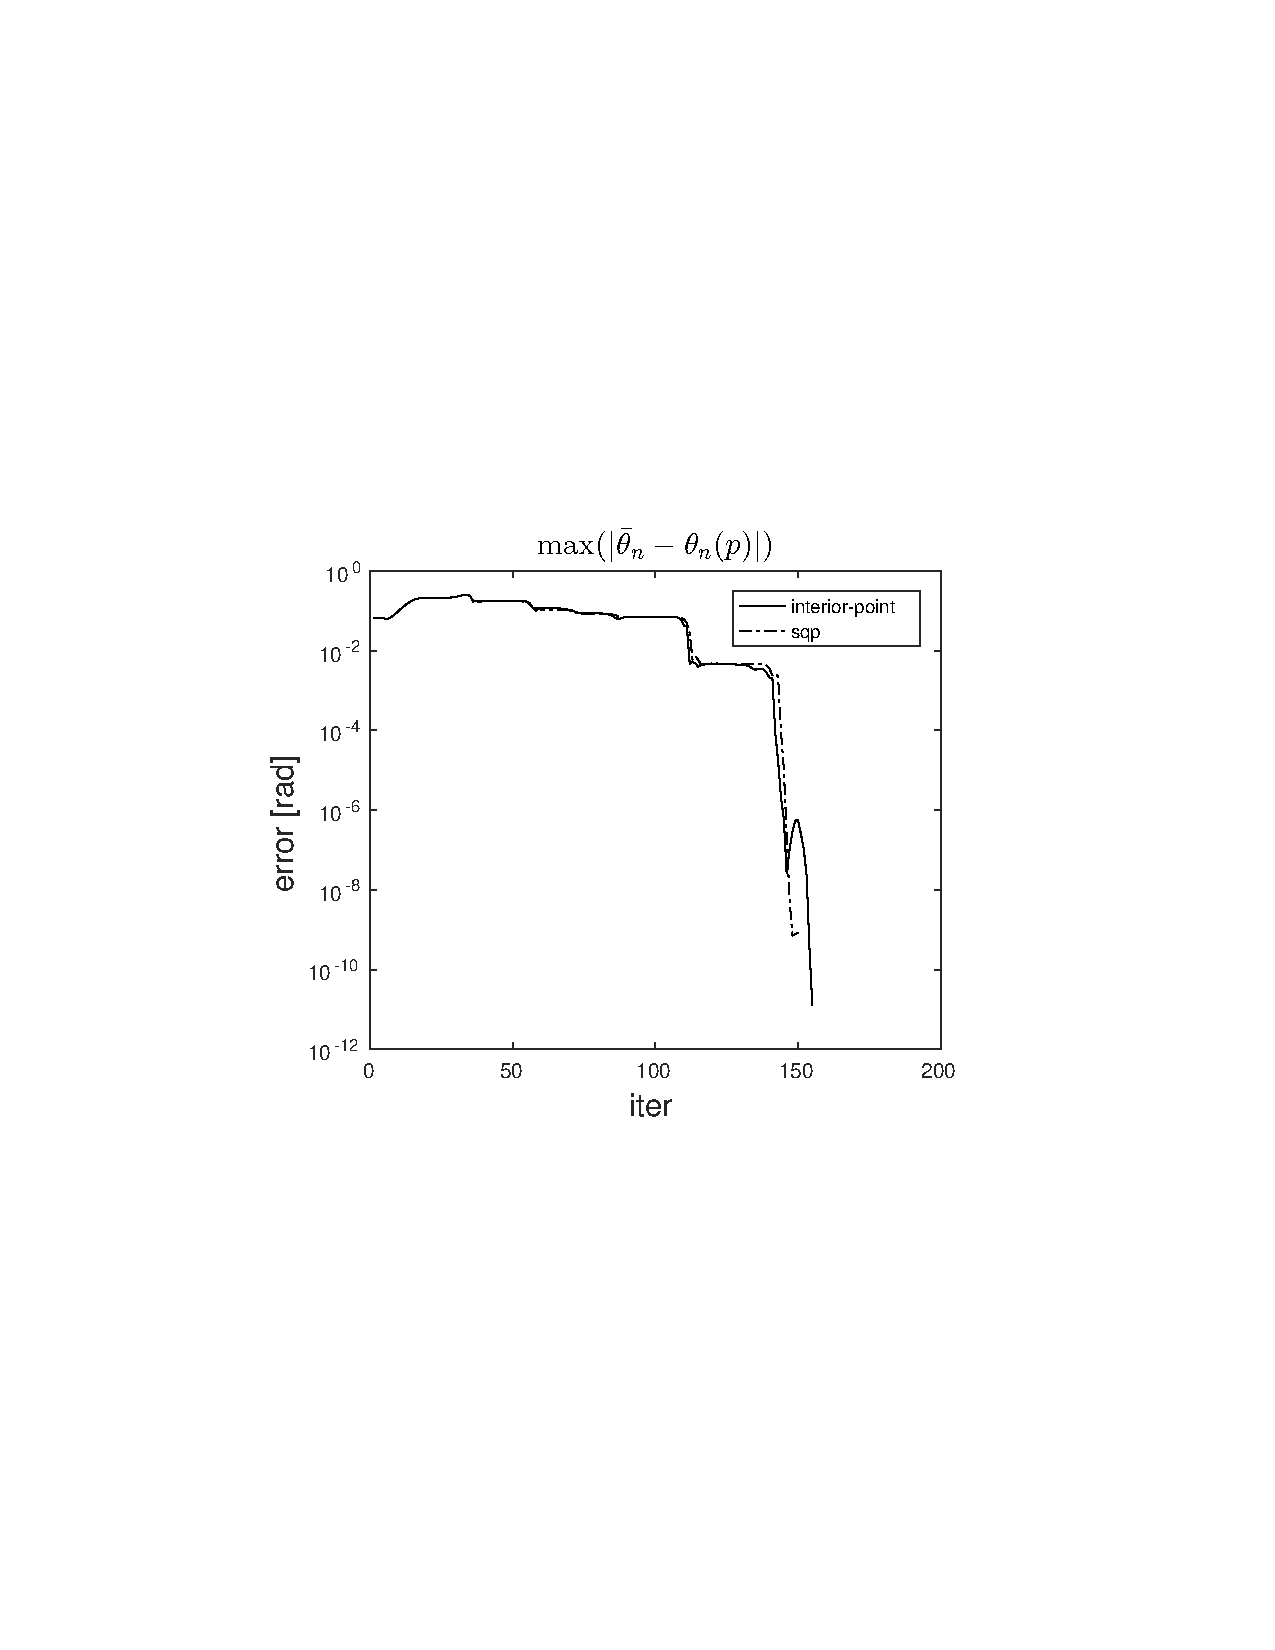
\includegraphics[trim=4cm 9cm 4cm 8.5cm, clip=true, width=\linewidth]{img/convPlotT_ref2}
            \end{figure}
    \end{columns}
\end{frame}

\begin{frame}
    \frametitle{Results}
    With approximation error

    \begin{columns}[t]
        \column{.5\linewidth}
            \begin{figure}
                \centering
                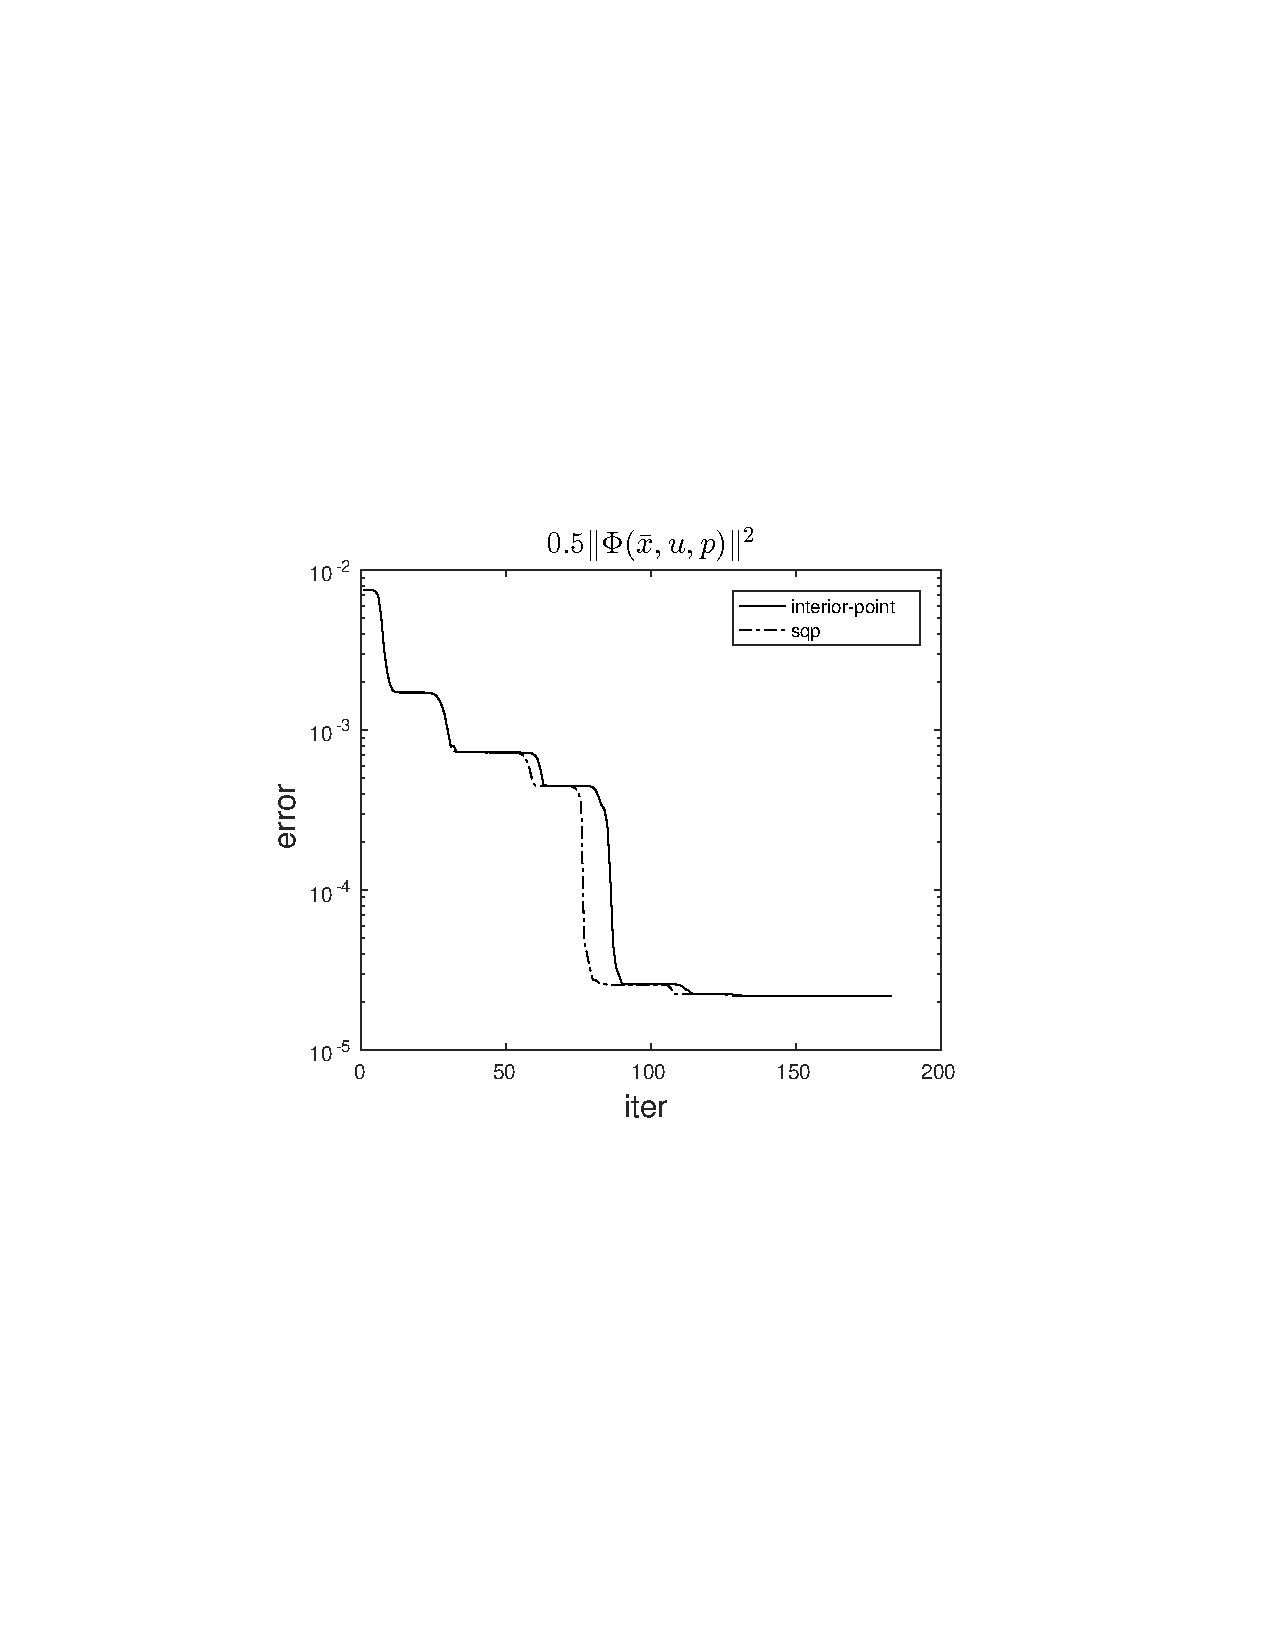
\includegraphics[trim=4cm 9cm 4cm 8.5cm, clip=true, width=\linewidth]{img/convPlotPhi_1}
            \end{figure}
        \column{.5\linewidth}
            \begin{figure}
                \centering
                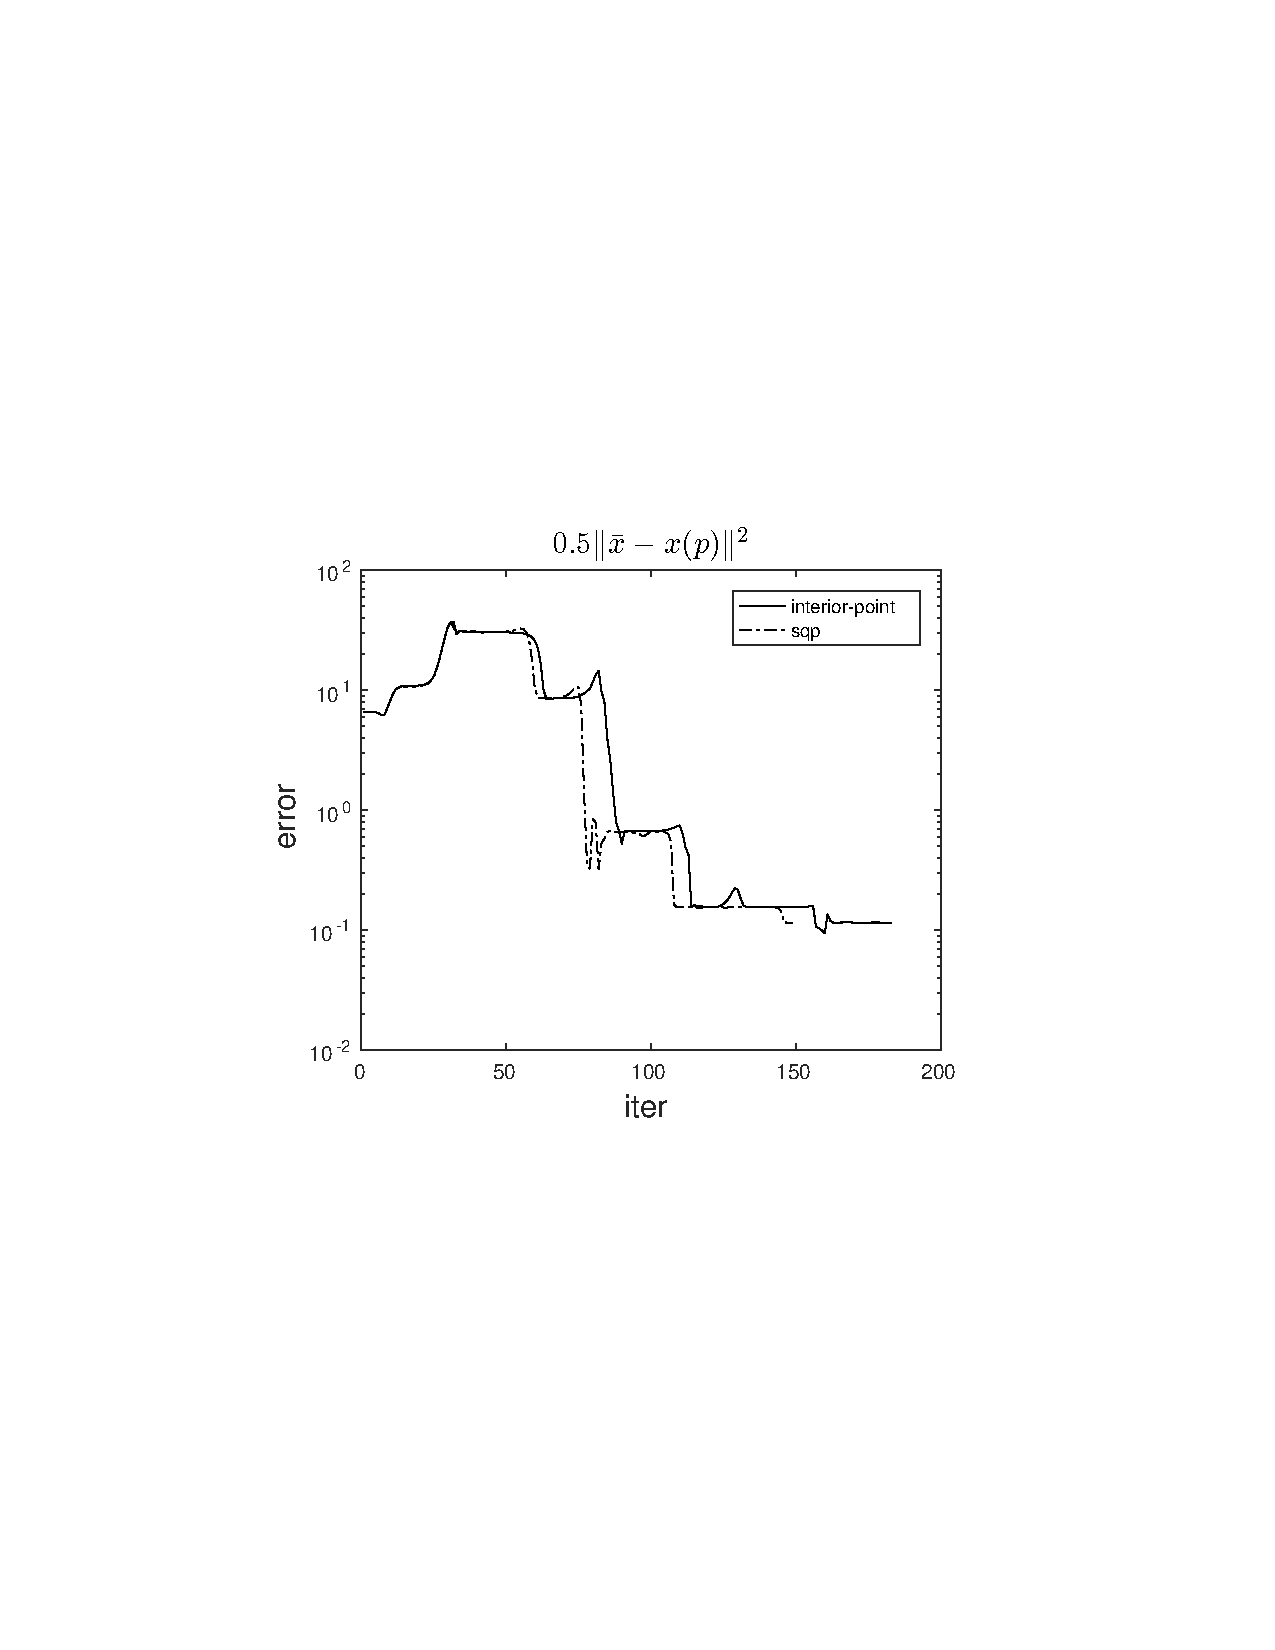
\includegraphics[trim=4cm 9cm 4cm 8.5cm, clip=true, width=\linewidth]{img/convPlotX_1}
            \end{figure}
    \end{columns}
\end{frame}

\begin{frame}
    \frametitle{Results}

    \begin{columns}[t]
        \column{.5\linewidth}
            \begin{figure}
                \centering
                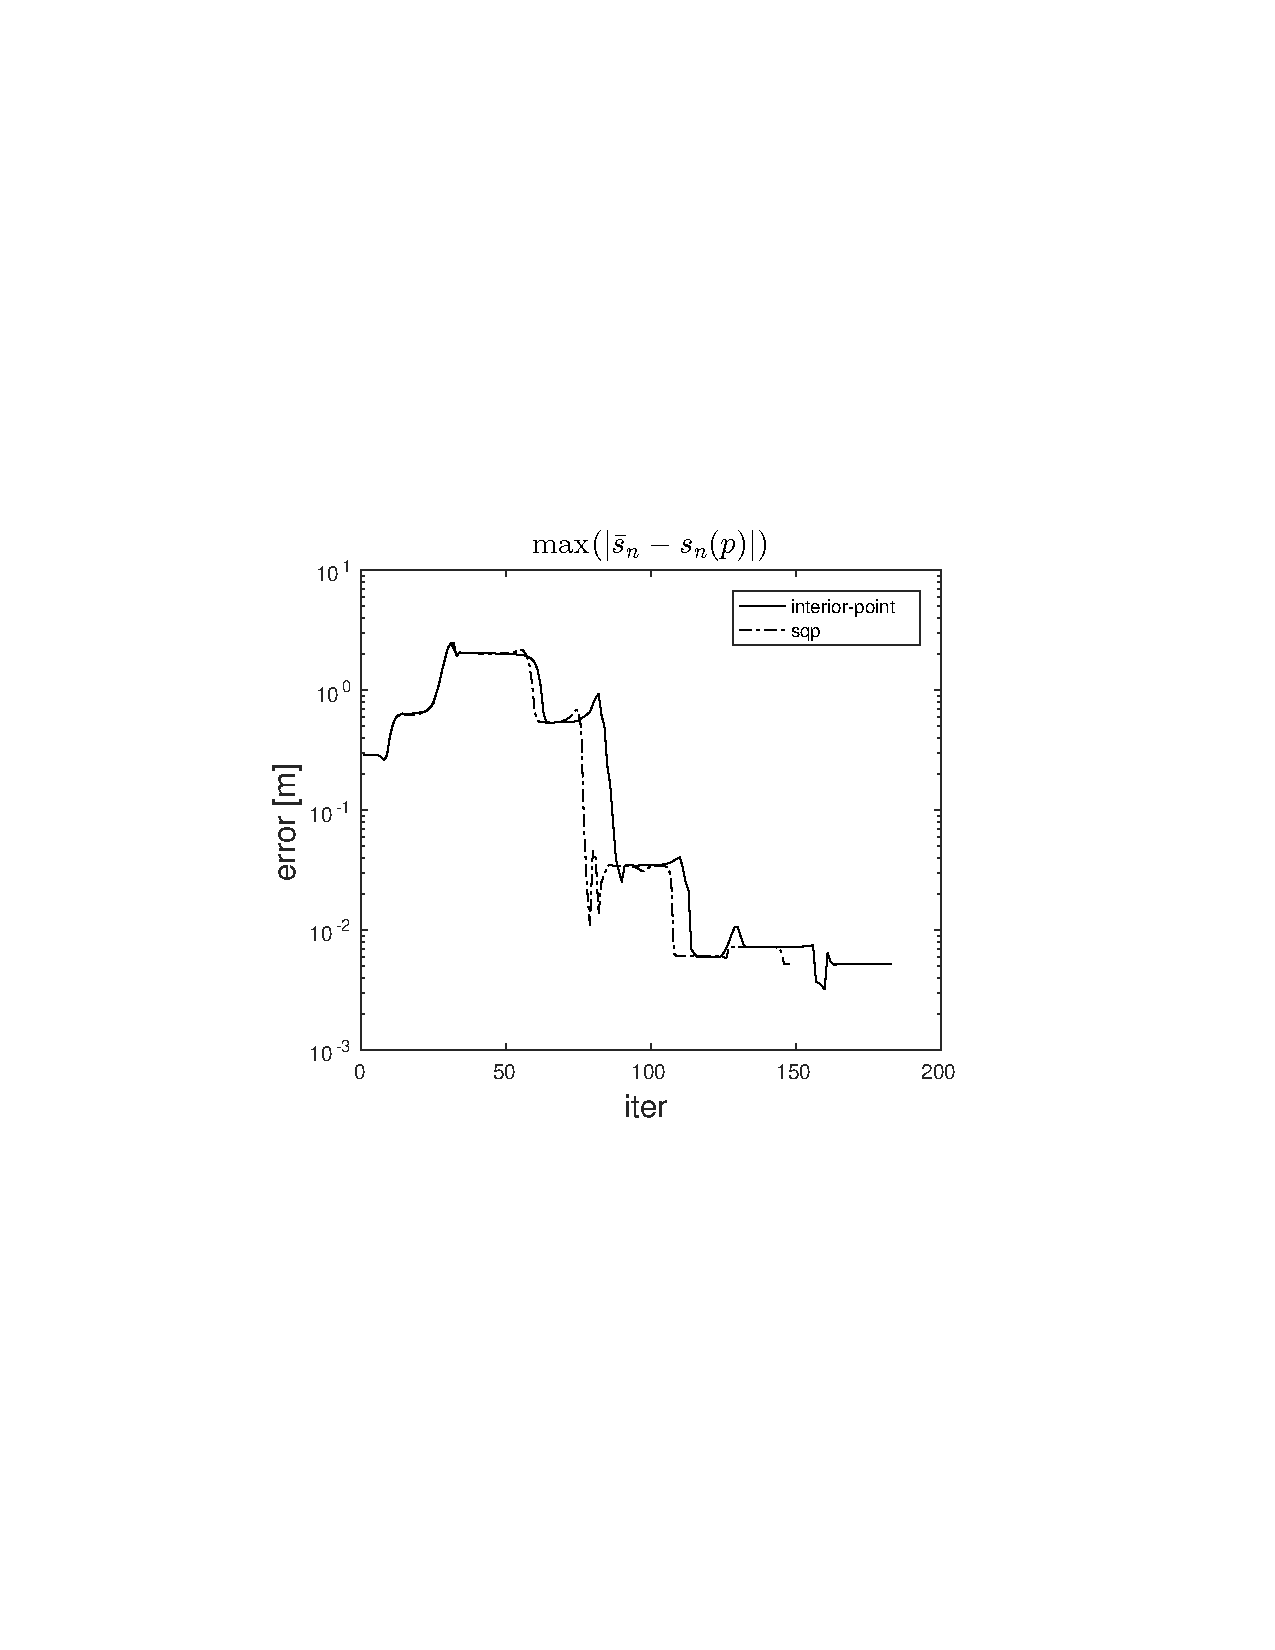
\includegraphics[trim=4cm 9cm 4cm 8.5cm, clip=true, width=\linewidth]{img/convPlotS_1}
            \end{figure}
        \column{.5\linewidth}
            \begin{figure}
                \centering
                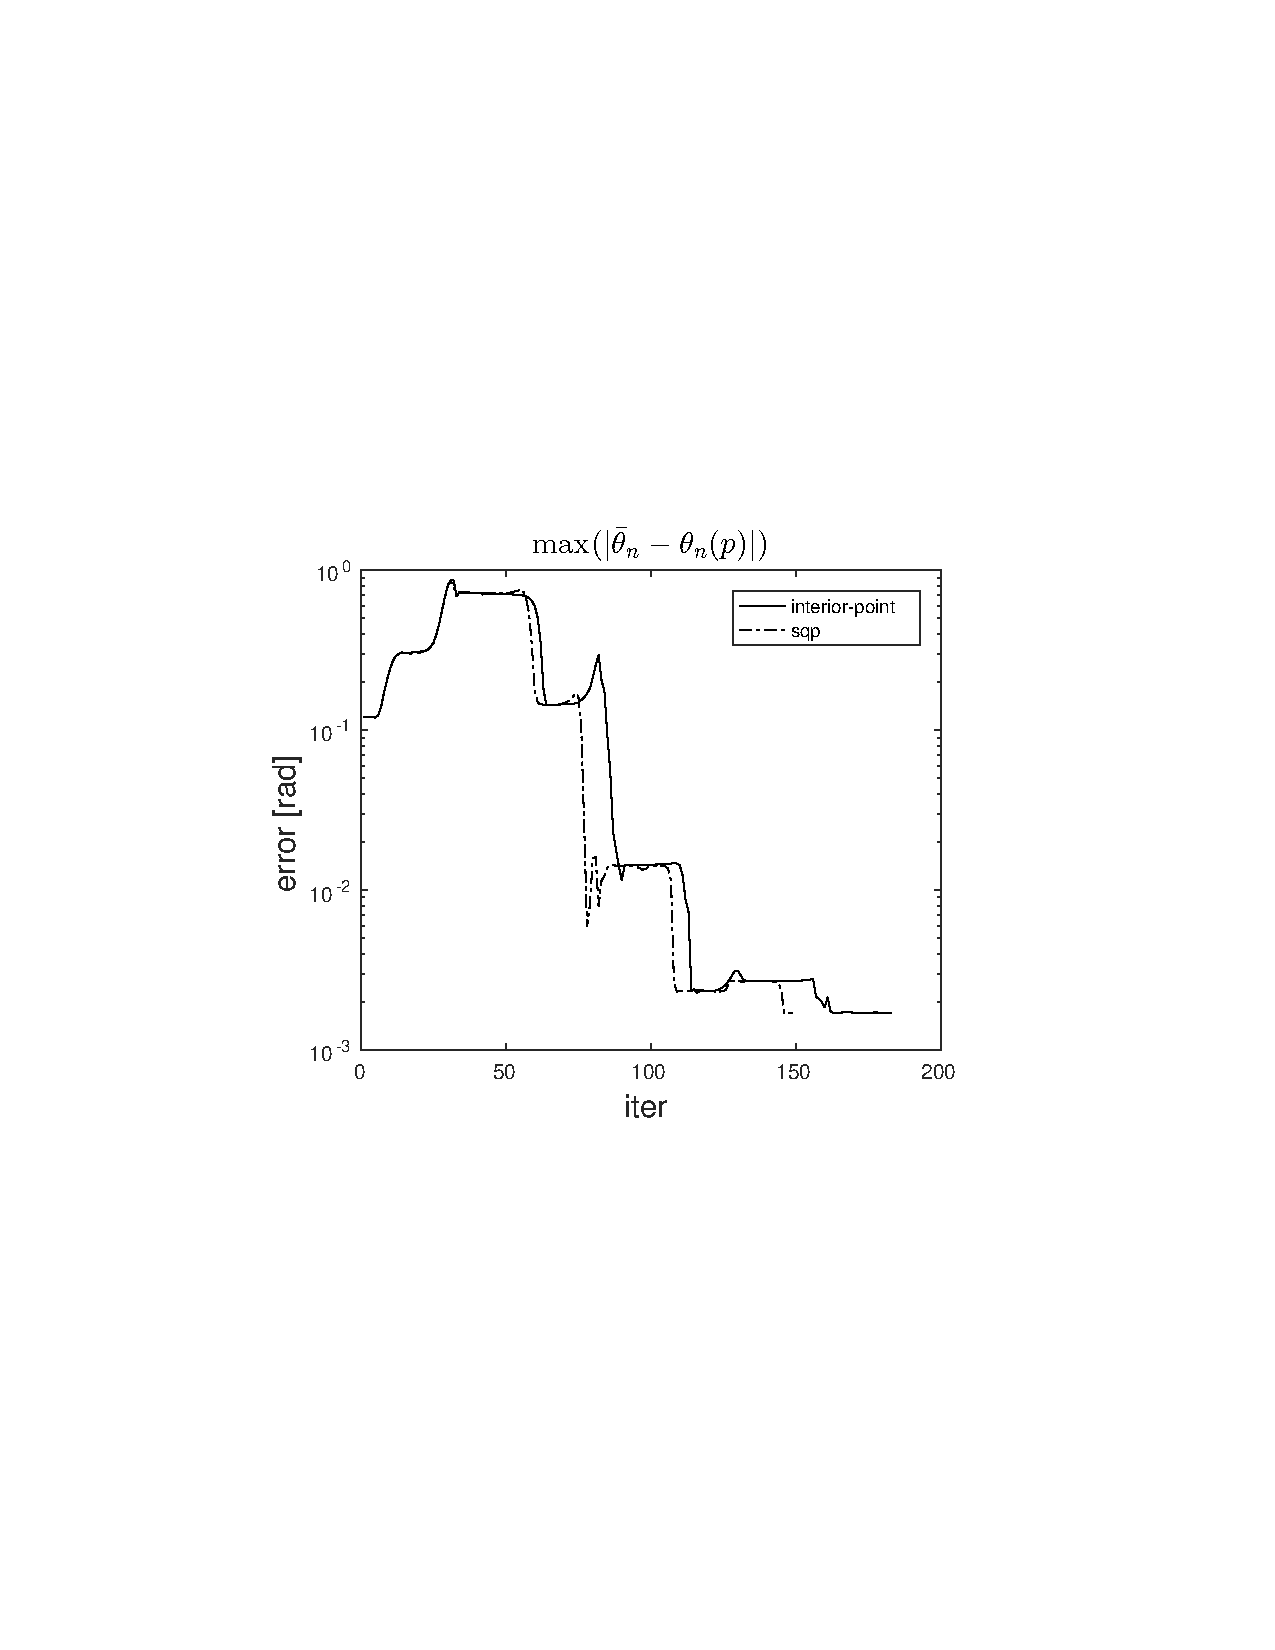
\includegraphics[trim=4cm 9cm 4cm 8.5cm, clip=true, width=\linewidth]{img/convPlotT_1}
            \end{figure}
    \end{columns}

    \begin{center}
        Exact up to $1\text{cm}$
    \end{center}
\end{frame}



\section{Black Box Model}
\begin{frame}[c]
	\frametitle{Test Run (1)}
	14 different cases:
	\begin{itemize}
		\item{Starting values: $N(\mu,\frac{\mu} 2), N(\mu,\frac{\mu}{20}), N(\mu,\frac{\mu}{200}), N(\frac{\mu}{10},\frac{\mu}{20}), N(10\mu,5\mu)$}
		\item{Swarm sizes: $4,10,40$}
		\item{Objective function: torques+positions, only positions}
		\item{4 solvers, each 5 loops per case}
	\end{itemize}
	Results:
	\begin{itemize}
		\item{Better values for "only position" (Particle Swarm: equal)}
		\item{Genetic Algorithm / Simulated Annealing better for good starting values, but much worse than Particle Swarm / Pattern Search}
		\item{Swarm Size changes have no effect}
		\item{Funccount independent from starting values, independent from objective function}
		\item{Time behaves as funccount}
	\end{itemize}
\end{frame}

\begin{frame}[c]
	\frametitle{Test Run (2)}
	5 different cases:
	\begin{itemize}
		\item{Starting values as before}
		\item{Solvers: Particle Swarm (torques + positions, only positions), Pattern Search (only positions)}
		\item{each 10 loops per case}
	\end{itemize}
	\vspace{.5cm}
	Results:
	\begin{itemize}
		\item{Starting values too big $\Rightarrow$ unrealistic results}
		\item{Similar results}
		\item{Particle Swarm is much faster}
		\item{Friction still hard to determine}
	\end{itemize}
\end{frame}

\begin{frame}[c]
	\frametitle{Results}
	Test Run (1)
	\begin{tabular}{l|lcrll}
		                    & value      & evaluations & time   & $\operatorname{dev}_{max}$ & $\operatorname{dev}_{mean}$ \\
		\hline
		Particle Swarm      & $10^{-12}$ & $2200$      & 6 min  & $10^{-1.0}$                & $10^{-3.8}$                 \\
		Pattern Search      & $10^{-11}$ & $6500$      & 17 min & $10^{-1.3}$                & $10^{-3.7}$                 \\
		Genetic Algorithm   & $10^{-4}$  & $5500$      & 14 min & $10^{-0.5}$                & $10^{-1.0}$                 \\
		Simulated Annealing & $10^{-3}$  & $4200$      & 11 min & $10^{-0.3}$                & $10^{-0.6}$                 \\
	\end{tabular} \\
	\vspace{.5cm}
	Test Run (2)
	\begin{tabular}{l|lcrll}
	                       & value      & evaluations & time   & $\operatorname{dev}_{max}$ & $\operatorname{dev}_{mean}$ \\
		\hline
		Particle Swarm (t+p) & $10^{-10}$ & $2900$      & 8 min  & $10^{-1.2}$                & $10^{-4.0}$                 \\
		Particle Swarm (p)   & $10^{-12}$ & $2000$      & 5 min  & $10^{-1.0}$                & $10^{-3.9}$                 \\
		Pattern Search (p)   & $10^{-12}$ & $6200$      & 17 min & $10^{-1.5}$                & $10^{-3.8}$                 \\
	\end{tabular}
\end{frame}

\end{document}
